\documentclass[../main.tex]{subfiles}

\pagestyle{main}
\renewcommand{\chaptermark}[1]{\markboth{\chaptername\ \thechapter:\ #1}{}}
\setcounter{chapter}{15}

\begin{document}




\chapter{Multiple Integrals}
\section{Double Integrals}
\begin{itemize}
    \item \marginnote{12/19:}\textbf{Double integral} (of $F(x,y)$ over the region $A$): The limit as $\Delta A\to 0$ of the sum of every $\Delta A_k$ (composing a region $A$) times $F(x,y)$ for some $(x,y)\in\Delta A_k$. Mathematically,
    \begin{equation*}
        \int_A\int F(x,y)\dd{A} = \lim_{\Delta A\to 0}\sum_{k=1}^nF(x_k,y_k)\Delta A_k
    \end{equation*}
    \begin{figure}[h!]
        \centering
        \begin{subfigure}[b]{0.4\linewidth}
            \centering
            \begin{tikzpicture}[
                every node/.append style={black}
            ]
                \footnotesize
                \draw [->] (-0.4,0) -- (5,0) node[right]{$x$};
                \draw [->] (0,-0.4) -- (0,4) node[above]{$y$};
                \foreach \x/\name in {0.5/a,4.5/b} {
                    \draw (\x,0.1) -- ++(0,-0.2) node[below]{$\name$};
                }
                \node [anchor=north east] {$O$};

                \fill [ylz] (2,1.5) rectangle (2.5,2);
                \draw [very thin] (0.2,0.6) grid[step=5mm] (4.7,3.7);
                \node at (2.25,2.2) {$\Delta x$};
                \node [text height=1.5ex,text depth=0.25ex] at (1.76,1.75) {$\Delta y$};

                \draw [ylx,thick,name path=f1] (0.3,1.2) to[out=-45,in=180] (1.8,0.8) to[out=0,in=-150,out looseness=0.3] node[pos=0.4,below right,fill=white,inner sep=1.5pt]{$y=f_1(x)$} (4.7,1.6);
                \draw [ylx,thick,name path=f2] (0.3,2.8) to[out=45,in=180] (1.8,3.2) to[out=0,in=150,out looseness=0.3] node[pos=0.4,above right,fill=white,inner sep=1.5pt]{$y=f_2(x)$} (4.7,2.4);
                \draw [ylx,semithick,name path=a] (0.5,3.7) -- (0.5,0.6);
                \draw [ylx,semithick,name path=b] (4.5,3.7) -- (4.5,0.6);

                \begin{scope}[on background layer]
                    \fill [
                        gay,
                        name intersections={of=f1 and a,by={f1a}},
                        name intersections={of=f1 and b,by={f1b}},
                        name intersections={of=f2 and b,by={f2b}},
                        name intersections={of=f2 and a,by={f2a}}
                    ] (f1a) to[out=-30,in=180] (1.8,0.8) to[out=0,in=-153,out looseness=0.3] (f1b) -- (f2b) to[out=153,in=0,in looseness=0.3] (1.8,3.2) to[out=180,in=30] (f2a);
                \end{scope}
            \end{tikzpicture}
            \caption{Subdividing the region $A$.}
            \label{fig:doubleIntegrala}
        \end{subfigure}
        \begin{subfigure}[b]{0.4\linewidth}
            \centering
            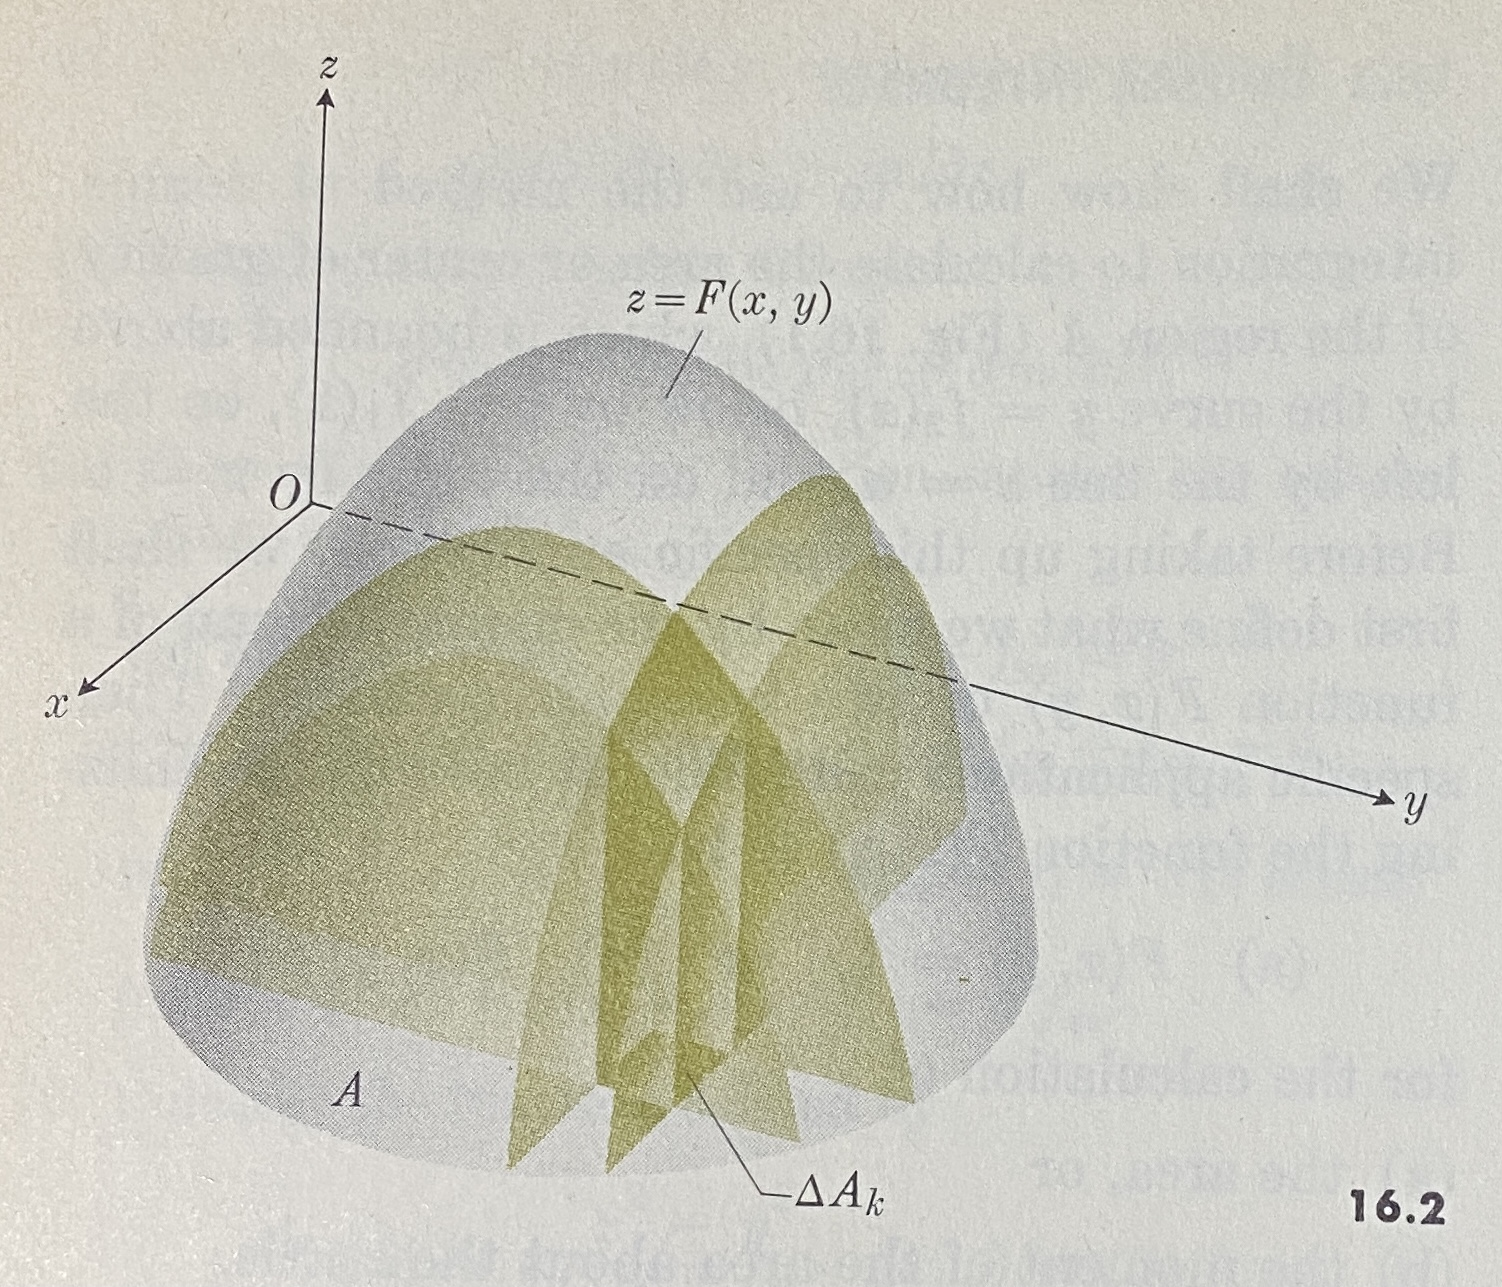
\includegraphics[width=0.9\linewidth]{ExtFiles/doubleIntegralb.jpg}
            \caption{Parts of $F(x,y)$ over a $\Delta A_k$.}
            \label{fig:doubleIntegralb}
        \end{subfigure}
        \caption{The double integral.}
        \label{fig:doubleIntegral}
    \end{figure}
    \begin{itemize}
        \item To conceptualize the double integral, first imagine that a region $A$ of the plane is bounded above by the curve $y=f_2(x)$, below by the curve $y=f_1(x)$, on the left by the line $x=a$, and on the right by the line $x=b$ (see Figure \ref{fig:doubleIntegrala}).
        \item Now imagine that $A$ is subdivided by a grid into $n$ pieces $\Delta A=\Delta x\Delta y=\Delta y\Delta x$. We disregard the pieces that lie partially or entirely outside of the bounds.
        \item As discussed in Chapter \ref{cht:15}, $F(x,y)$ can be thought of as a surface in three-space. For the sake of simplicity, we will imagine for right now that $F(x,y)$ is positive for all $(x,y)\in A$, i.e., that it lies above $A$ (see Figure \ref{fig:doubleIntegralb}).
        \item With this picture, we can imagine summing the partial volumes $F(x,y)\cdot\Delta A_k$ for each $\Delta A_k$ where $(x,y)$ is some point in $\Delta A_k$ to approximate the total volume under the surface (analogous to the area under the curve).
        \item All that the double integral does at this point is find the exact volume under the surface by taking the limit of this summation as we consider increasingly more increasingly small slivers of volume.
    \end{itemize}
    \item We can evaluate the double integral of $F(x,y)$ over $A$ if $F(x,y)$ is continuous throughout $A$, if the boundary curves are continuous and have finite total length, and if we let $\Delta y=2\Delta x$ (or some other similar function) and let $\Delta x\to 0$.
    \item To evaluate double integrals, we calculate one or the other of the \textbf{iterated} integrals\footnote{Proving that evaluating these integrals is equivalent to evaluating the double integral is a more advanced theorem of analysis.}
    \begin{align*}
        \int_A\int F(x,y)\dd{x}\dd{y}&&
            \int_A\int F(x,y)\dd{y}\dd{x}
    \end{align*}
    \item To evaluate the latter integral above, for example, we integrate \dq{$\int F(x,y)\dd{y}$ with respect to $y$ (with $x$ held fixed) and [evaluate] the resulting integral between the limits $y=f_1(x)$ and $y=f_2(x)$, and then [integrate] the result\dots with respect to $x$ between the limits $x=a$ and $x=b$}{549} Mathematically,
    \begin{equation*}
        \int_A\int F(x,y)\dd{y}\dd{x} = \int_a^b\left( \int_{f_1(x)}^{f_2(x)}F(x,y)\dd{y} \right)\dd{x}
    \end{equation*}
    \begin{figure}[h!]
        \centering
        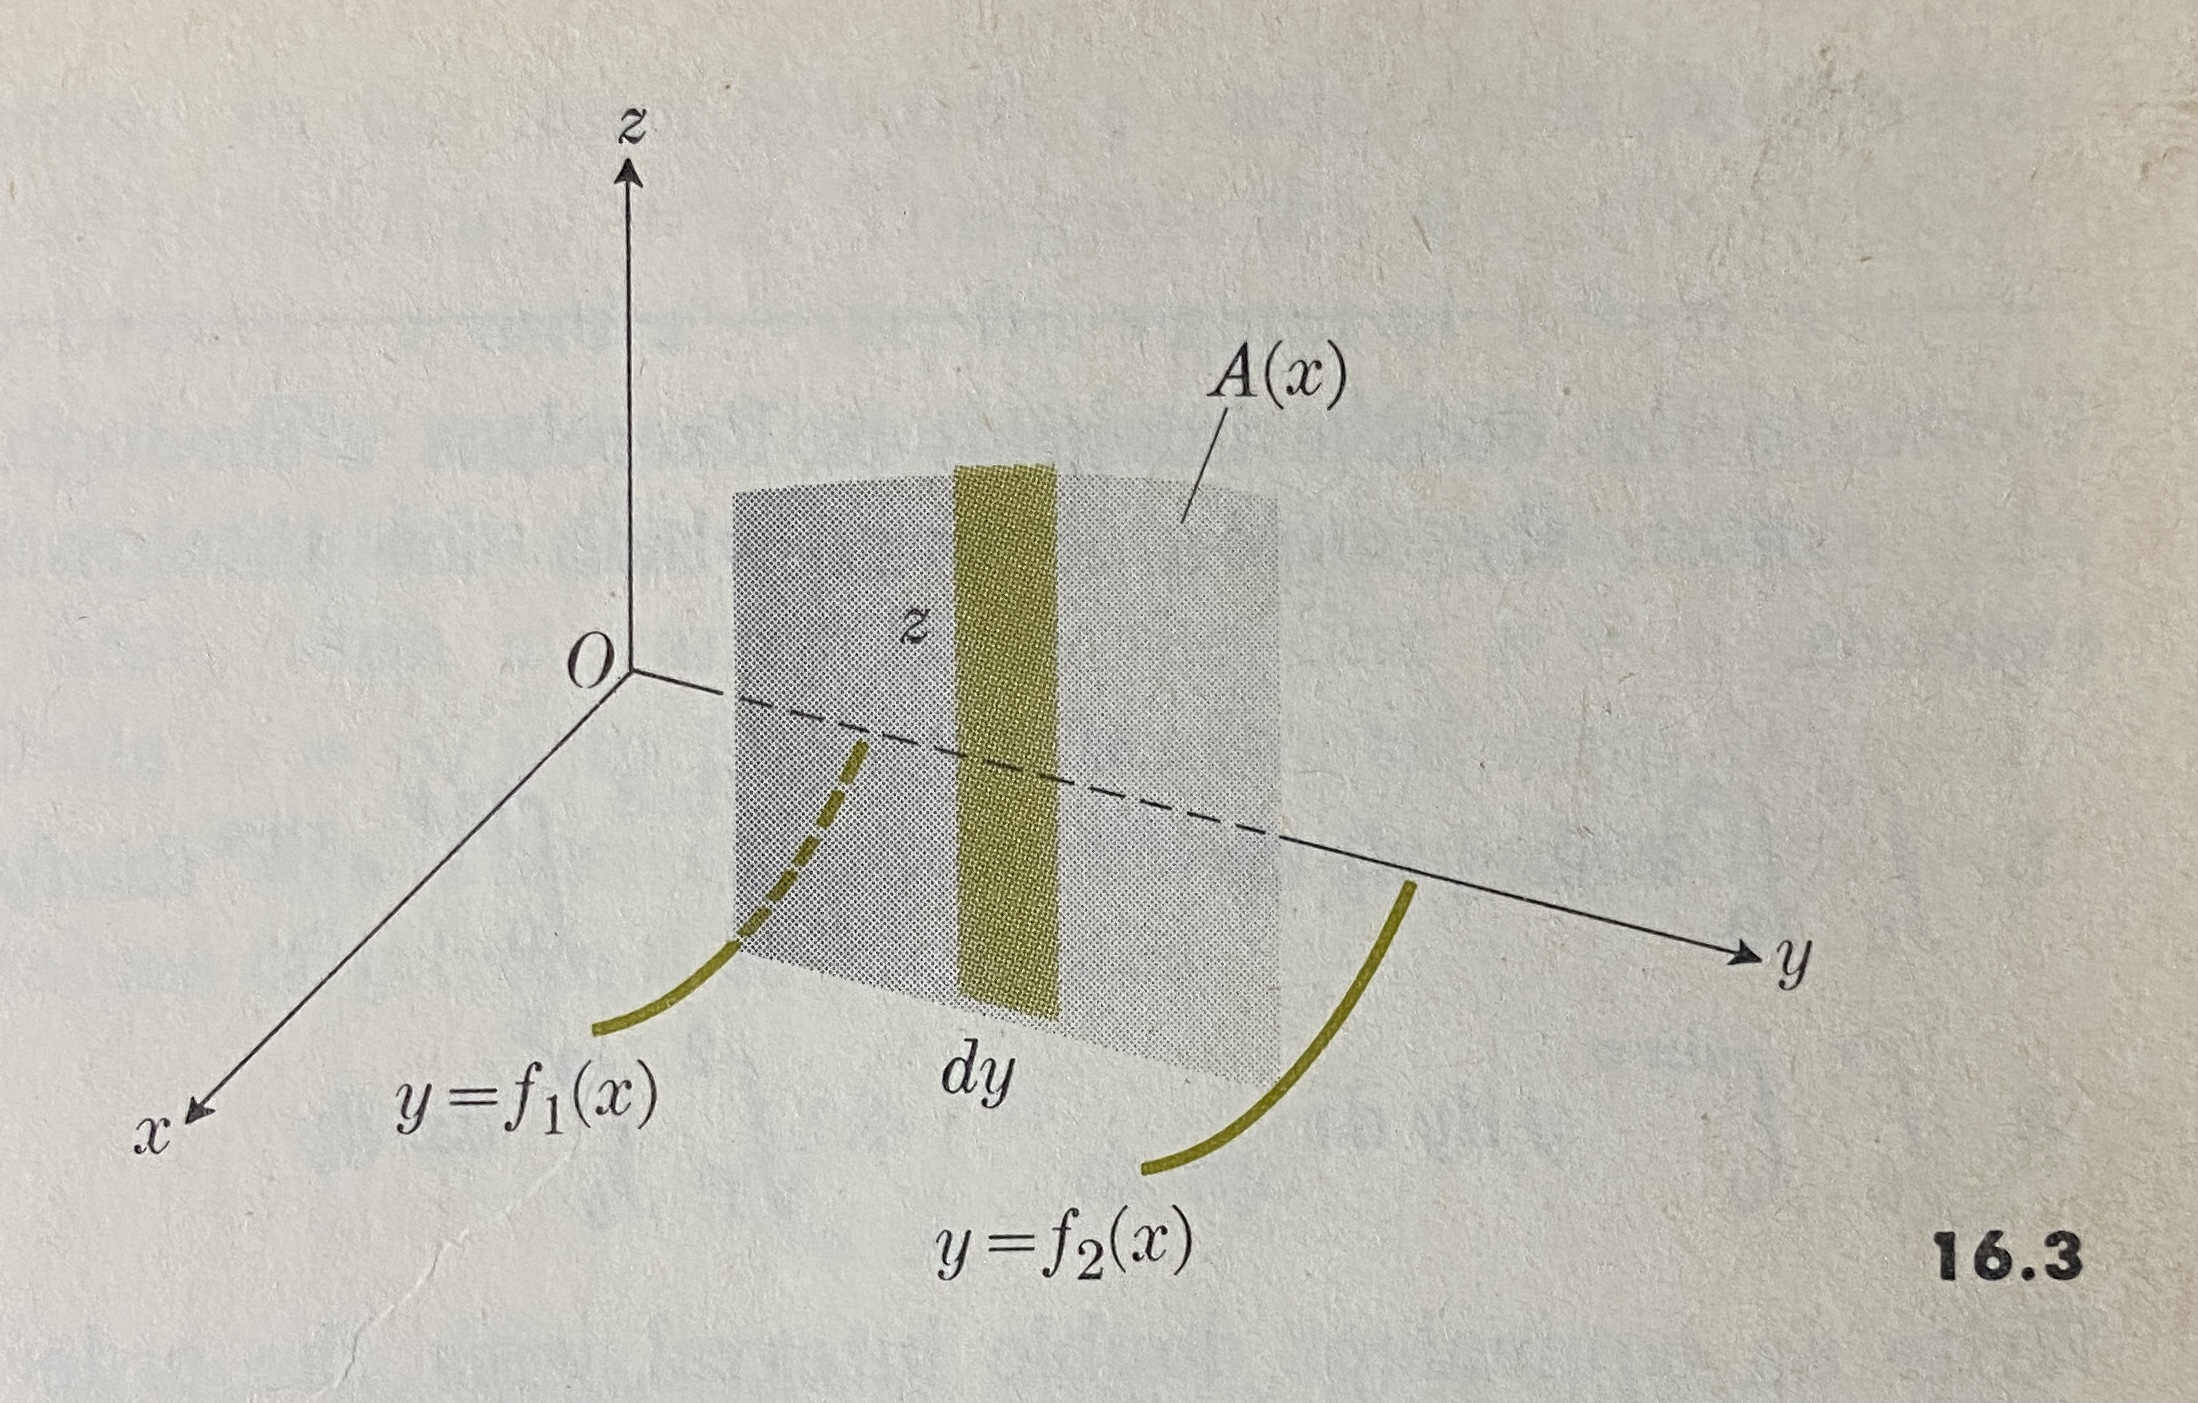
\includegraphics[width=0.4\linewidth]{ExtFiles/interatedIntegration.jpg}
        \caption{Visualizing iterated integration.}
        \label{fig:iteratedIntegration}
    \end{figure}
    \begin{itemize}
        \item To visualize iterated integration, imagine determining the volume under the surface by summing infinitely many infinitely thin cross sections of the solid parallel to the $y$-axis.
        \item The cross section at $x=x_0$ would have area $A(x_0)=\int_{f_1(x_0)}^{f_2(x_0)} F(x_0,y)\dd{y}$.
        \item The sum of all such cross sections' contributions to the volume would be the integral $\int_a^bA(x)\dd{x}=\int_a^b\left( \int_{f_1(x)}^{f_2(x)} F(x,y)\dd{y} \right)\dd{x}$.
    \end{itemize}
\end{itemize}



\section{Area by Double Integration}
\begin{itemize}
    \item The area of the region of the $xy$-plane is given by either of the following integrals (with proper limits of integration).
    \begin{equation*}
        A = \iint\dd{x}\dd{y} = \iint\dd{y}\dd{x}
    \end{equation*}
    \item In cases such as that of Figure \ref{fig:doubleIntegrala}, it makes sense to integrate with respect to $y$ first and $x$ second. However, if we have a region bounded by $y=c$, $y=d$, $x=g_1(y)$, and $x=g_2(y)$, then it would make more sense to do the opposite.
    \item Conceptualize the iterated integration here as summing the infinitesimal areas of strips parallel to the $x$- or $y$-axis, the lengths of which are given by $f_2(x)-f_1(x)=\int_{f_1(x)}^{f_2(x)}\dd{y}$ or $g_2(y)-g_1(y)=\int_{g_1(y)}^{g_2(y)}\dd{x}$.
\end{itemize}




\end{document}